\documentclass[11pt,czech,american,dvipsnames]{book}
\usepackage[T1]{fontenc}
\usepackage[utf8]{inputenc}
\usepackage[a4paper]{geometry}
\geometry{verbose,tmargin=4cm,bmargin=3cm,lmargin=3cm,rmargin=2cm,headheight=0.8cm,headsep=1cm,footskip=0.5cm}
\pagestyle{headings}
\setcounter{secnumdepth}{3}
\usepackage{url}
\usepackage{amsmath}
\usepackage{mathtools}
\usepackage{amsthm}
\usepackage{amssymb}
\usepackage{amstext}
\usepackage{graphicx}
\usepackage{setspace}
\usepackage{wrapfig}
\usepackage{algorithm}
\usepackage{algpseudocode}
\usepackage{svg}
\usepackage{outlines}
\usepackage[normalem]{ulem}
\usepackage{dirtytalk}
% \usepackage{subcaption}
% \usepackage{subfigure}

\usepackage{xargs}                      % Use more than one optional parameter in a new commands
\usepackage{xcolor}  % Coloured text etc.
\usepackage[colorinlistoftodos,prependcaption,textsize=tiny]{todonotes}
\newcommandx{\unsure}[2][1=]{\todo[linecolor=red,backgroundcolor=red!25,bordercolor=red,#1]{#2}}
\newcommandx{\change}[2][1=]{\todo[linecolor=blue,backgroundcolor=blue!25,bordercolor=blue,#1]{#2}}
\newcommandx{\info}[2][1=]{\todo[linecolor=OliveGreen,backgroundcolor=OliveGreen!25,bordercolor=OliveGreen,#1]{#2}}
\newcommandx{\add}[2][1=]{\todo[linecolor=Plum,backgroundcolor=Plum!25,bordercolor=Plum,#1]{#2}}
\setlength{\marginparwidth}{1.75cm}

\makeatletter
\newenvironment{lyxlist}[1]
{\begin{list}{}
{\settowidth{\labelwidth}{#1}
 \setlength{\leftmargin}{\labelwidth}
 \addtolength{\leftmargin}{\labelsep}
 \renewcommand{\makelabel}[1]{##1\hfil}}}
{\end{list}}

\usepackage[varg]{txfonts}

\usepackage{indentfirst}

\clubpenalty=9500

\widowpenalty=9500

\hyphenation{CDFA HARDI HiPPIES IKEM InterTrack MEGIDDO MIMD MPFA DICOM ASCLEPIOS MedInria}

\renewcommand{\vec}[1]{\boldsymbol{#1}}
\newcommand{\code}{\texttt}

\newtheorem{thm}{Theorem} % [section]
\newtheorem{lem}{Lemma}
\newtheorem{prop}{Proposition}
\newtheorem{cor}{Corollary}
\newtheorem{conj}{Conjecture}
\newtheorem{dfn}{Definition}

\DeclareMathOperator{\id}{id}
\DeclareMathOperator*{\argmax}{arg\,max}
\DeclareMathOperator*{\argmin}{arg\,min}
\DeclarePairedDelimiter{\ceil}{\lceil}{\rceil}

% \DeclarePairedDelimiter\ceil{\lceil}{\rceil}
% \DeclarePairedDelimiter\floor{\lfloor}{\rfloor}

\def\code#1{\texttt{#1}}

\newcommand{\bd}[1]{\mathbf{#1}}
\newcommand{\RR}{\mathbb{R}}      
\newcommand{\ZZ}{\mathbb{Z}}
\newcommand{\ZZP}{\mathbb{Z}+^}
\newcommand{\NN}{\mathbb{N}}
\newcommand{\QQ}{\mathbb{Q}}
\newcommand{\CC}{\mathbb{C}}
\newcommand{\col}[1]{\left[\begin{matrix} #1 \end{matrix} \right]}
\newcommand{\comb}[2]{\binom{#1^2 + #2^2}{#1+#2}}
\newcommand{\Tau}{\mathrm{T}}
\newcommand*\diff{\mathop{}\!\mathrm{d}}

\DeclarePairedDelimiter\norm{\lVert}{\rVert}
\interfootnotelinepenalty=10000 % ! THIS MAY CAUSE TROUBLE !

\makeatother

\usepackage{babel}

\begin{document}

\title{Removed sections}
\author{Miroslav Kovář}
\date{\today}
\maketitle

\chapter{Convolutional Neural Networks}

\section{Mathematical background}
TODO: Do we really need this section???

\begin{dfn}
  Let $I$ be an image function, $K$ a kernel. A (discrete) \textbf{convolution} of $I$ and $K$ is a functional defined as
  \begin{align}
    (I*K)(i,j) = \sum_m \sum_n I(m,n) K(i-m, j-n) \, .
  \end{align}
\end{dfn}

Note that some machine learning libraries (such as Tensorflow) implement \textbf{cross-correlation} instead of convolution, but preserving the term convolution for the operation. Cross-correlation corresponds to convolution with kernel rotated by 90 degrees:
\begin{align}
  (I*K)(i,j) = \sum_m \sum_n I(m,n) K(i+m, j+n) \, .
\end{align}
Unlike convolution, cross-correlation is not commutative, but this property is not required for neural network applications.

\begin{dfn}
  Let $f$ be arbitrary function, and $\mathcal{D}$ its degradation operator. We say $f$ is \textbf{invariant} under $\mathcal{D}$ if
  \begin{align}
    \mathcal{D}(f) \equiv f \, .
  \end{align}
\end{dfn}

For the following, the reader needs to understand the term \textbf{equivariance}. 
\begin{dfn}[\cite{pitts2013}]
  Let $G$ be a group and $X$, $Y$ its G-sets. Then $F:X \rightarrow Y$ is called an \textbf{equivariant function} if
  \begin{align}
    F(g(x)) = g(F(x))
  \end{align}
  for all $G$ actions $g$ and $x \in X$.
\end{dfn}

For our purposes, we can view $G$ as a group of transformations, and then equivariance as a commutative property of a function with regards to the transformations. In other words, computing the function and then applying the transformation has the same effect as applying the transformation and then computing the function.

TODO: This is probably too basic to be here

\textbf{Gradient descent} is a first order iterative method of finding an extremum a differentiable function $f : \RR \rightarrow \RR^n$, $f \in C^1$, based on continually moving a point in its domain in the direction of negative of its gradient at that point, until the absolute value of the gradient (or the step size) is below a certain threshold. See Algorithm \ref{alg:gd}.

\begin{algorithm}
  \caption{Gradient descent algorithm.}
  \label{alg:gd}
\begin{algorithmic}[1]
  \State Initialize random $x_0 \in D(f)$
  \State $n \gets 0$
  \State step\_size $\gets 1$  
  \While{step\_size $ < \text{threshold}$ and $n < $ iters\_limit}
  \State $x_{n+1} = x_n - \epsilon \nabla_{x_n} f$
  \State step\_size $\gets |x_{n+1} - x_n|$ 
  \State $n \gets n + 1$
  \EndWhile
\end{algorithmic}
\end{algorithm}

\textbf{Stochastic gradient descent}\dots

\section{History}

The classical approach to image pattern recognition consists of the following stages:
\begin{description}
  \item[preprocessing:] supressing unwanted distortions and noise, enhancement beneficient for further processing,
  \item[object segmetation:] separating disparate objects from the background,
  \item[feature extraction:] gathering relevant information about the properties of the objects, removing irrelevant variations,
  \item[classification:] categorizing segmented objects based on obtained features into classes.
\end{description}

The preprocessing step may require additional assumptions about the data or further processing, which are potentially too restrictive or too broad. Getting around this limitation requires dealing with complications such as high dimensionality of the input (number of pixels) and desirability of invariance towards a number of allowable distortions and geometrical transformations.

Artificial neural networks in combination with gradient-based learning are one possible solution to the problem. By gradually optimizing a set of weights based on a training data set using a differentiable error function, they provide a framework for learning a suitable set of assumptions automatically from the data.

One of the oldest neural network architectures, fully connected multi-layer perceptron (FC-MLP), can be used for image pattern recognition. However, it has the following drawbacks:
\begin{description}
  \item[parameter explosion:] the number of parameters of such network is exponential in the number of layers, increasing the capacity of the network and therefore need for more data,
  \item[no invariance:] no invariance even with respect to common geometrical transformation such as translation, rotation and scaling,
  \item[ignoring input topology:] natural ../Images exhibit strong local structure and high correlation between intensities of neighboring pixels, but FC-MLPs are unstructed - inputs can be presented in any order.
\end{description}

Although the main idea dates back to 1980, when K. Fukushima introduced neocognitron \cite{fukushima1982}, the back-propagation algorithm was not known at the time. The first convolutional architecture successfuly applied on an image pattern recognition problem by attempting to solve the aforementioned problems, dubbed LeNet-5, was proposed in 1998 by Y. LeCun, L. Bottou, Y. Bengio and P. Haffner \cite{LeCun1998}.

\section{Description}

\begin{figure} 
\centering
\noindent\makebox[\textwidth]{%
  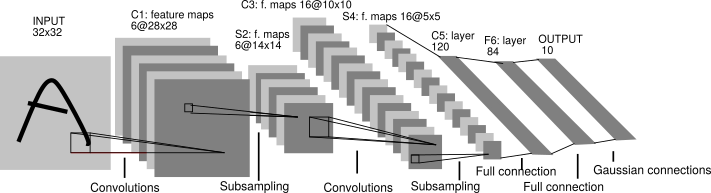
\includegraphics[width=0.8\textwidth]{../Images/lenet-5.png} }
  \caption{LeNet-5 architecture \cite{lecun1999}.}
\label{fig:lenet-5}
\end{figure}

Bearing resemblence to visual processing in biological organisms \footnote{As early as in 1968, D. H. Hubel and T.N. Wiesel discovered that some cells (called simple cells) in cat's primary visual cortex (V1) with small receptive fields (shared by neighboring neurons) are sensitive to straight lines and edges of light of particular orientation, and other cells (called complex cells) with larger receptive fields further in the visual cortex also respond to straight lines and edges, but with invariance to translation \cite{Hubel1968}.}, LeNet-5 proposed the following design principles to enforce \emph{shift, scale and distortion invariance}: \cite{lecun1999}
\begin{description}
  \item[local receptive fields:] each neuron in a layer receives input from a small neighborhood in the previous layer,
  \item[shared weights:] each layer is composed of neurons organized in planes within which each neuron have the same weight vector (feature map),
  \item[spatial subsampling:] adding a subsampling layers, which reduce the resolution of the previous layer by averaging or taking the maximal value of neighboring pixels in the previous layer.
\end{description}

\subsection{Local receptive fields}
\emph{Local receptive fields} enable the network to synthesize filters that produce strong response to elementary salient features in the early layers (such as lines, edges and corners in a visual input, and their equivalents in other modalities), and then learn to combine them in the subsequent layers to produce higher-order feature detectors.

\begin{figure} 
\centering
\noindent\makebox[\textwidth]{%
  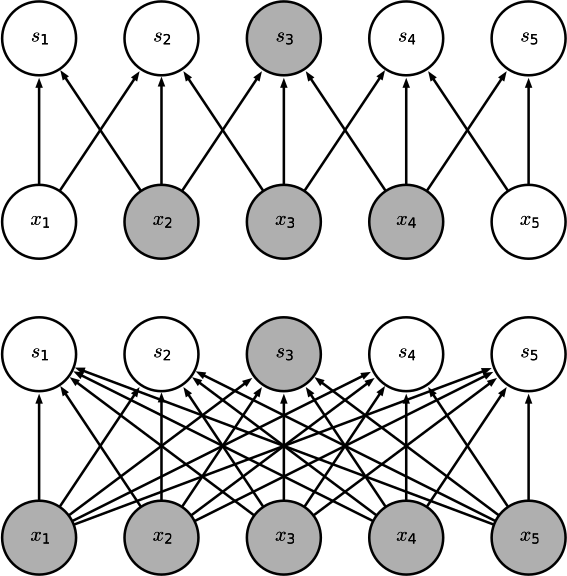
\includegraphics[width=0.5\textwidth]{../Images/receptive_field.png} }
  \caption{Receptive field. \cite{goodfellow2016}}
\label{fig:receptive_field}
\end{figure}

For a visual explanation of the concept of receptive field, see Figure \ref{fig:receptive_field}. The locality of of those receptive fields implies sparser connectivity, and hence more efficient computations in comparison with fully connected neural networks. A fully connected neural network with no hidden layers with $m$ inputs and $n$ outputs has $m \times n$ weight parameters, and the correspoding feed forward pass (matrix multiplication) is of $O(m \times n)$ time complexity per input. If the number of connections per output unit is limited to $k < m$, the achieved runtime is $O(k \times n)$, where $k$ is usally in practice several orders of magintude smaller than $m$. \cite{goodfellow2016}

In shallow neural networks, locality of receptive fields implies locality of ``influence'' of each input unit on the output. In deep neural networks, on the other hand, units in the deeper layers can be indirectly connected to some or all units of the input, thus enabling them to achieve aforementioned effect of combining more complex features from simpler ones.

\subsection{Shared weights}
With \emph{shared weights}, neural units in a layer with differing receptive fields have the same feature map and the same feature detecting operation (convolution with feature map kernel followed by additive bias and a application of a non-linear function) is performed on differing parts of the image (see Figure \ref{fig:shared_weights}). A single convolutional layer is composed of multiple feature detecting planes.

Shared weights principle exploits the fact that in natural ../Images, a function of small number of neighboring pixels can be useful in multiple parts of the image. For example, an edge detector can be used accross the entire image to detect edges in the first layer, an object detector can then be used to detect presence of edges in particular arrangements in the next layer, etc.

Although it does not reduce the time complexity of the feedforward pass, it does reduce the memory requirements. If the kernel size is $k$, $m$ the number of inputs, $n$ the number of outputs, the number of parameters per layer is $k$ instead of $m \times n$ (per feature detecting plane) in a fully connected case. Since $k$ is usually in practice several orders of magnitude smaller than $m$, and usually $m$ and $n$ are comparable in size, the memory savings are highly significant. \cite{goodfellow2016}

One of the drawbacks of classical CNNs is that although convolution in combination with weight sharing causes layer output to be equivariant to translation of the input, this is not the case for scaling and rotation. Moreover, equivariance to input may not be always desirable. Consider a case of face detection, where all training and test ../Images are centered. Then, the relative positions of individual features are important, and it may be favorable to fix feature detectors (and thus weights) to certain locations in the image.

\subsection{Pooling}
\begin{figure} 

\centering
\noindent\makebox[\textwidth]{%
  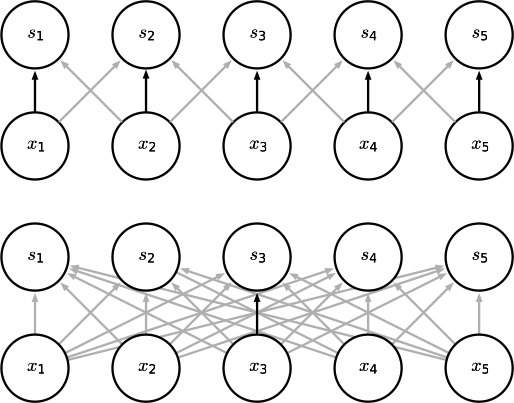
\includegraphics[width=0.5\textwidth]{../Images/shared_weights.png} }
  \caption{Shared weights. \cite{goodfellow2016}}
\label{fig:shared_weights}
\end{figure}

The final output activations of a convolutional layer are computed in subsequent stages:
\begin{enumerate}
  \item linear unit activations are computed via the convolution operation,
  \item a non-linear activation function is applied to the activations,
  \item a spatial subsampling (pooling) operation is applied.
\end{enumerate}

The rationale behind applying a non-linearity is it makes the network capable of modelling non-linear functions. Common activation functions include rectified linear $\max(0,x)$, sigmoid $\frac{1}{1+\exp(-x)}$, hyperbolic tangent $\tanh$, and many others. They have varying properties making them useful in different situations. We will not explore them further here.

\emph{Pooling} operation splits the neural units into sets of multiple adjacent activations and computes a summary statistic, such as the maximum element (max pooling) or the average (average pooling), per such set and outputs the result. If the stride between the sets is greater than one, the spatial dimension of output is decreased relative to input (subsampling).

The purpose of spatial subsampling is to ensure scale and distortion invariance\footnote{Whether it achieves this goal has been famously doubted by Geoffrey Hinton: ``The pooling operation used in convolutional neural networks is a big mistake and the fact that it works so well is a disaster.'' \cite{}} by reducing the precision at which a feature is encoded in a feature map by reducing its resolution - when scale and distortion invariance is assumed, the exact location of a feature becomes less important and is allowed to exhibit slight positional variance - roughly speaking, an ``approximate'' translation invariance.

Although the combination of convolution and pooling performs well in many practical situations, it has multiple drawbacks. For example, the learned representations are not rotation invariant and thus, to mitigate this, the capacity of the network has to be increased and the training dataset must be enhanced to contain examples of rotated features, often extending the amount of data necessary and training time. A number of alternative approaches were suggested in the litarature.\footnote{For instance, Hinton's \emph{CapsNet}, described e.g. in \cite{sabour2017}, is an attempt to transform the manifold of ../Images of similar shape (which is highly non-linear in the space of pixel intensities) to a space where it is globally linear by the way of using so called capsules instead of traditional convolutional layers.} For another example of a limitation, see Figure \ref{fig:drawbacks}.

\begin{figure} 
\centering
\noindent\makebox[\textwidth]{%
  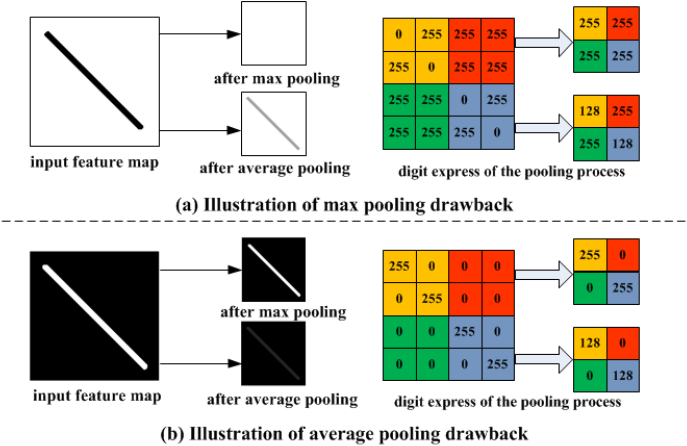
\includegraphics[width=0.8\textwidth]{../Images/drawbacks.png} }
  \caption{Examples of drawbacks of the pooling operation. Max pooling discards all except the maximum element, and valuable information may thus be lost. Average pooling considers all the values, and the information about their contrast is reduced. Moreover, extreme values may have undesired effects on the result. \cite{yu2014}}
\label{fig:drawbacks}
\end{figure}


\section{Applications}
Maybe mention an example of how LeNet-5 was improved on subsequently (AlexNet, ResNet, etc.)? But this changes all the time\dots

\section{CapsNets?} \label{sec:capsnets}
Does it make sense trying them? I found a only a few successful implementations. Maybe it would be better to try those after we have some results already, because it seems risky - we might end up with nothing.

\chapter{Dynamical systems}
\section{Visual characterization of the dynamical system}
\subsection{Phase space plot}
\subsection{Poincare plot}
\subsection{Recurrence plot}
When presented with a task of finding regularities in seemingly chaotic data, one possible approach is analysing at least approximate repetitions of simple patterns, which can be further used for reconstruction of more complicated rules. Recurrence plot is a method of visualizing obtained state-space trajectory segments in relation to each other to achieve this goal. Furthermore, it can be used to test necessary conditions for validity of dynamical parameters derivable from a non-linear time series such as the information dimension, entropy, Lyapunov exponents, dimension spectrum, etc. The information contained in recurrence plots is not easily obtainable by other known methods. \cite{eckmann1987}

\begin{dfn}[\cite{eckmann1987}]
  Let $N$ be the length of given time series, $\mathbf{s}_i$ for $i \in \{1,2,\dots,N \}$ be a $i$-th delay vector of any integer embedding dimension, $\norm{\cdot}$ a norm, $\Theta(\cdot)$ a Heaviside step function, and $\epsilon \in \RR_0^+$ a tolerance parameter. Then, \textbf{recurrence plot} is the matrix
  \begin{align}
    M_{ij} = \Theta(\epsilon - \norm{ \textbf{s}_i - \textbf{s}_j }) \, .
  \end{align}
\end{dfn}

In other words, $M_{ij}$ is a symmetric\footnote{Although this is true for our definition, it may not be true for an alternative definition using a more general topology instead of a norm.} binary $N x N$ matrix, where $M_{ij} = 1$ when $i$-th and $j$-th points of the reconstructed trajectory enter each other's $\epsilon$ neighborhood.

The essential drawback of recurrence plot is their size - it is quadratic in the length of the time series. A simple way of reducing its dimension is to partition the time series into disjoined segments, and let $M_{ij}$ represent the distance between those two segments. This is known as \textbf{meta-recurrence plot}. \cite{kantz2004} (TODO: Find a justification for using them.)

(TODO: Cross-recurrence plots may be useful? Only between two series. Joint recurrence plots may be used to detect phase synchronization.)

\bibliographystyle{plain}
\bibliography{../refs}
\end{document}
